\setcounter{section}{30}\setcounter{dang}{0}
\section{ĐỊNH NGHĨA VÀ Ý NGHĨA CỦA ĐẠO HÀM}
\subsection{KIẾN THỨC CẦN NHỚ}
\subsubsection{Định nghĩa đạo hàm tại một điểm}
\begin{enumerate}[\iconMT]
	\item \indam{Định nghĩa:} Cho hàm số $y=f(x)$ xác định trên $(a;b)$ và $x_0 \in (a;b)$. Nếu giới hạn $\lim\limits_{x\to x_0}\dfrac{f(x)-f(x_0)}{x-x_0}$ \textbf{hữu hạn} thì kết quả đó được gọi là đạo hàm của hàm số $y=f(x)$ tại điểm $x_0$. Kí hiệu $f'(x_0)$ hay $y'(x_0)$. Tức là
		\boxmini{$f'(x_0)=\lim\limits_{x\to x_0}\dfrac{f(x)-f(x_0)}{x-x_0}$  $\quad (2)$}
	\item \indam{ Lưu ý:}
	\begin{itemize}
		\item Đại lượng $\Delta x =x-x_0$ được gọi là số gia của biến tại $x_0$.
		\item Đại lượng$\Delta y =f(x)-f(x_0)=f(x_0+\Delta x)-f(x_0)$ được gọi là số gia tương ứng của hàm số.
	\end{itemize}
	Khi đó công thức (2) được viết thành 
		\boxmini{$f'(x_0)=\lim\limits_{\Delta x \to 0}\dfrac{\Delta y}{\Delta x}$ $\quad (3)$} 
	\begin{note}
		Muốn tính đạo hàm tại một điểm cho trước, ta chọn một trong hai công thức (2) hoặc (3).
	\end{note}
\end{enumerate}

\subsubsection{Đạo hàm trên một khoảng}
Hàm số $y=f(x)$ được gọi là có đạo hàm trên khoảng $(a;b)$ nếu nó có đạo hàm tại mọi điểm  $x$ trên khoảng đó. Kí hiệu $y'$ hoặc $f'(x)$

\subsubsection{Ý nghĩa vật lý của đạo hàm}
\begin{itemize}
	\item [\iconMT] \indam{Vận tốc tức thời:}  Xét chuyển động thẳng xác định bởi phương trình $s=f\left( t \right)$, với $f\left( t \right)$ là hàm số có đạo hàm. Khi đó, vận tốc tức thời của chất điểm tại thời điểm $t_0$ là đạo hàm của hàm số $s=f\left( t \right)$ tại $t_0$. Nghĩa là
	$$v\left( t_0 \right)=s'\left(t_0 \right)=f'\left(t_0 \right).$$
	\item [\iconMT] \indam{Cường độ tức thời:} Điện lượng $Q$ truyền trong dây dẫn xác định bởi phương trình $Q=f\left( t \right)$, với $f\left( t \right)$ là hàm số có đạo hàm. Khi đó, cường độ tức thời của dòng điện tại thời điểm $t_0$ là đạo hàm của hàm số $Q=f\left( t \right)$ tại $t_0$. Nghĩa là 
	$I\left( t_0 \right)=Q'\left( t_0 \right)=f'\left( t_0 \right).$
\end{itemize}

\subsubsection{Ý nghĩa hình học của đạo hàm}
\immini{Cho hàm số $y=f(x)$ xác định trên $(a;b)$ và có đạo hàm tại $x_0 \in (a;b)$. Gọi $\mathscr{(C)}$ là đồ thị của hàm số đó. Ta có hai kết quả sau:
\begin{note}
	\begin{itemize}
		\item [\ding{172}] $f'(x_0)$ là hệ số góc của tiếp tuyến $\Delta$ của đồ thị $\mathscr{(C)}$ tại điểm $M(x_0;y_0)$.
		\item [\ding{173}] Phương trình tiếp tuyến $\Delta \colon y-y_0=f'(x_0)(x-x_0)$.
		\begin{itemize}
			\item $(x_0;y_0)$ là tọa độ tiếp điểm;
			\item $f'(x_0)$ là hệ số góc của tiếp tuyến.
		\end{itemize}
	\end{itemize}
\end{note}}{
	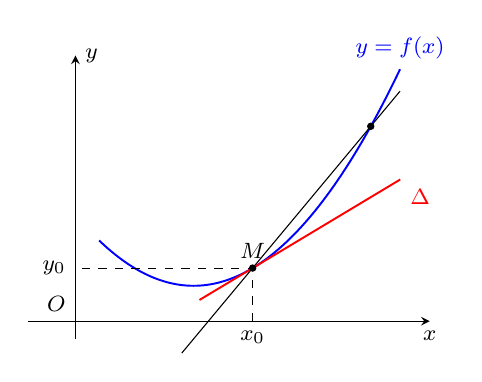
\begin{tikzpicture}[smooth,samples=300,scale=0.75,y=0.6cm,>=stealth,font=\footnotesize]
	\draw[->] (-0.8,0)--(6,0) node[below]{$x$};
	\draw[->] (0,-0.5)--(0,7.5) node[right]{$y$};
	\draw (0,0) node[above left]{$O$};
	\draw[line width=0.7pt,domain=0.4:5.5,blue] plot(\x,{0.5*(\x-2)^2+1})node[above]{$y=f(x)$};
	\draw[line width=0.4pt,domain=1.8:5.5] plot(\x,{2*(\x)-4.5});
	\draw[line width=0.7pt,domain=2.1:5.5,red] plot(\x,{(\x)-1.5})node[below right]{$\Delta$};
	\draw[fill=black] (3,1.5) circle(1.5pt) (5,5.5) circle(1.5pt);
	\draw[dashed] (3,0)node[below]{$x_0$}--(3,1.5)node[above]{$M$}--(0,1.5)node[left]{$y_0$};
	%\node[right] at (2,2.4) {$2$};
	\end{tikzpicture}}

\subsubsection{Quan hệ giữa sự tồn tại đạo hàm và tính liên tục}
[\iconMT] \indam{Định lý:} Nếu hàm số  $y=f(x)$  có đạo hàm tại điểm $x_0$   thì nó liên tục tại điểm đó.

\subsection{PHÂN LOẠI VÀ PHƯƠNG PHÁP GIẢI TOÁN}

\begin{dang}{Tính đạo hàm của hàm số y = f(x) tại một điểm}
	Chọn một trong hai cách:
	\begin{enumerate}[\iconCH]
		\item \indamm{Cách 1:}
		\begin{itemize}
			\item [$\bullet$] Tính $\lim\limits_{x\to x_0}\dfrac{f(x)-f(x_0)}{x-x_0}$;
			\item [$\bullet$] Nếu giới hạn này hữu hạn và có kết quả là $a$, thì ta kết luận $f'(x_0)=a$.
		\end{itemize}
		\item \indamm{Cách 2:}
		\begin{itemize}
			\item [$\bullet$] Tính $\Delta y=f(x_0+\Delta x)-f(x_0)$ và tính giới hạn $\lim\limits_{\Delta x \to 0}\dfrac{\Delta y}{\Delta x}$;
			\item [$\bullet$] Nếu giới hạn này hữu hạn và có kết quả là $a$, thì ta kết luận $f'(x_0)=a$.
		\end{itemize}
	\end{enumerate}
\end{dang}

\begin{vd}%[Khuất Văn Thanh]%[1D5B1]
	Tính đạo hàm của hàm số $y=-x^2$ tại điểm $x_0=2$ bằng định nghĩa.
	\loigiai{
	}
\end{vd}\dongcham{3}

\begin{vd}%[1D5B1-1]
	Tính đạo hàm của các hàm số sau tại các điểm đã sau:
	\begin{tasks}(1)
		\task $f(x)=2x^2+x+1$ tại $x=2$;
		\task $f(x)=x^3$ tại $x=3$;
		\task $f(x)=\sqrt{x}$ tại $x=4$;
		\task $f(x)=\sqrt{2x+1}$ tại $x=1$;
	\end{tasks}
	\loigiai{
		
	}
\end{vd}\dongcham{20}

\begin{vd}
	Tính đạo hàm của hàm số số $y=x(x-1)(x-2) \ldots(x-2021)$ tại điểm $x=0$.
	\loigiai{
		Ta có $f^{\prime}(0)=\lim _{x \rightarrow 0} \frac{f(x)-f(0)}{x-0}=\lim _{x \rightarrow 0} \frac{x(x-1)(x-2) \ldots(x-2021)}{x}$
		
		$$
		=\lim _{x \rightarrow 0}(x-1)(x-2) \ldots(x-2021)=(-1) \cdot(-2) \ldots(-2021)=-2021!
		$$
	}
\end{vd}
\dongcham{7}
\begin{vd}
	Tính đạo hàm (nếu tồn tại) của hàm số $y=|x-1| x^2$ tại điểm $x_0=1$.
	\loigiai{
		Đạo hàm $y(1)$ (nếu có) là
		$$
		y^{\prime}(1)=\lim _{x \rightarrow 1} \dfrac{y-0}{x-1}=\lim _{x \rightarrow 1} \dfrac{|x-1| x^2}{x-1} .
		$$
		Ta cần tính riêng các giới hạn bên phải và bên trái tại điểm 1. Ta có
		$$
		\begin{aligned}
			& \lim _{x \rightarrow 1^{+}} \dfrac{|x-1| x^2}{x-1}=\lim _{x \rightarrow 1^{+}} \dfrac{(x-1) x^2}{x-1}=\lim _{x \rightarrow 1^{+}} x^2=1 \\
			& \lim _{x \rightarrow 1^{+}} \dfrac{|x-1| x^2}{x-1}=\lim _{x \rightarrow 1^{-}} \dfrac{-(x-1) x^2}{x-1}=\lim _{x \rightarrow 1^{+}}\left(-x^2\right)=-1 .
		\end{aligned}
		$$
		Giới hạn bên phải và bên trái tại điểm 1 khác nhau nên không tồn tại giới hạn $\lim _{x \rightarrow 1} \dfrac{|x-1| x^2}{x-1}$. Do đó, đạo hàm $y^{\prime}(1)$ không tồn tại.\\
		\textbf{Chú ý}. $|x-1| x^2=(x-1) x^2$ khi $x \geq 1$ và $|x-1| x^2=-(x-1) x^2$ khi $x<1$ nên để khử vô định trong giới hạn trên ta phải xét riêng các giới hạn một phía.
	}
\end{vd}\dongcham{7}

\begin{vd}
Một chất điểm chuyển động có phương trình chuyển động là: $s=f(t)=t^2+4 t+6$ ( t được tính bằng giây, s được tính bằng mét)
\begin{enumEX}[a)]{1}
	\item Tính đạo hàm của hàm số $f(t)$ tại điểm $t_0$.
	\item Tính vận tốc tức thời của chuyến động tại thời điếm $t=5$.
\end{enumEX}
\loigiai{
\begin{enumerate}[a)]
	\item Ta có: $\lim _{t \rightarrow t_0} \frac{f(t)-f\left(t_0\right)}{t-t_0}=\lim _{t \rightarrow t_0} \frac{t^2+4 t+6-\left(t_0^2+4 t_0+6\right)}{t-t_0}==\lim _{t \rightarrow t_0}\left(t+t_0+4\right)=2 t_0+4$.
	
	Vậy $f^{\prime}\left(t_0\right)=2 t_0+4$.
	\item Vận tốc tức thời của chuyển động tại thời điểm $t=5$ là $v_{t t}=f^{\prime}(5)=2.5+4=14(\mathrm{~m} / \mathrm{s})$.
\end{enumerate}
}
\end{vd}
\dongcham{7}

\begin{dang}{Viết phương trình tiếp tuyến của đồ thị hàm số tại điểm cho trước}
\end{dang}


\begin{vd}%[1D7N1-1]
	Cho hàm số $y=(2 x+1)^2$.
	\begin{enumerate}
		\item  Bằng định nghĩa, hãy tính đạo hàm của hàm số đã cho tại điểm $x_0=-1$.
		\item  Viết phương trình tiếp tuyến của đồ thị hàm số tại điểm $A(-1 ; 1)$.
	\end{enumerate}
	
	\loigiai{
		\begin{enumerate}
			\item  Tại điểm $x_0=-1, y_0=(-2+1)^2=1$. Với $x \neq-1$, ta có:\\ $$\dfrac{y-1}{x-(-1)}=\dfrac{(2 x+1)^2-1}{x+1}=\dfrac{(2 x+1-1)(2 x+1+1)}{x+1}=2 \cdot 2 x.$$ Do đó: $y^{\prime}(-1)=\lim \limits_{x \to-1} \dfrac{y-1}{x-(-1)}=\lim \limits_{x \to-1} 2 \cdot 2 x=-4$.
			\item  Phương trình tiếp tuyến của đồ thị hàm số tại điểm $A(-1 ; 1)$ là: $$ y-1=y^{\prime}(-1)(x-(-1))=-4(x+1) \text { hay } y=-4 x-3$$
		\end{enumerate}
	}
\end{vd}\dongcham{9}%

\begin{vd}%[1D7N1-1]
	Cho hàm số $y=x^3$.
	\begin{enumerate}
		\item  Bằng định nghĩa, hãy tính đạo hàm của hàm số đã cho tại điểm $x_0$ bất kì ($x_0 \in \mathbb{R}$).
		\item  Viết phương trình tiếp tuyến của đồ thị hàm số tại điểm $M(-2;-8)$.
	\end{enumerate}
	\loigiai{
	}
\end{vd}\dongcham{8}%

\begin{vd}%[1D7N1-1]
	Cho hàm số $y=\sqrt{x}$.
	\begin{enumerate}
		\item  Bằng định nghĩa, hãy tính đạo hàm của hàm số đã cho tại điểm $x_0>0$ bất kì.
		\item  Viết phương trình tiếp tuyến của đồ thị hàm số tại điểm có hoành độ bằng 4.
	\end{enumerate}
	\loigiai{
	}
\end{vd}\dongcham{9}%

\begin{dang}{Ý nghĩa vật lý của đạo hàm}
	\begin{enumerate}[\iconCH]
		\item Xét chuyển động thẳng xác định bởi phương trình $s=s(t)$, trong đó $s$ là quảng đường đi được trong thời gian $t$. Lúc đó, vận tốc tức thời của chuyển động tại thời điểm $t_0$ là $v(t_0)=s'(t_0)$.
		\item Ý nghĩa tổng quát: Đạo hàm của một hàm số chính là đặc trưng cho tốc độ thay đổi của hàm số theo biến số của nó.
	\end{enumerate}
\end{dang}
\begin{vd}
	Một vật rơi tự do theo phương trình $s=\dfrac{1}{2}gt^2$, trong đó $g\approx 9,8\mathrm{\, m/s^2}$ là gia tốc trọng trường. Tìm vận tốc tức thời của chuyển động tại thời điểm $t_0=5\mathrm{\,s}$.
	\loigiai{Ta có: $v(t_0)=s'(t_0)=\lim\limits_{t\rightarrow t_0}\dfrac{s(t)-s(t_0)}{t-t_0}=\lim\limits_{t\rightarrow t_0}\dfrac{\frac{1}{2}gt^2-\frac{1}{2}gt_0^2}{t-t_0}=gt_0$. Do đó, tại thời điểm $t_0=5\mathrm{\,s}$ vận tốc tức thời của chuyển động là $v(5)=5g\approx 49\mathrm{\, m/s}$.
	}
\end{vd}\dongcham{6}


\subsection{BÀI TẬP TỰ LUYỆN}

\begin{bt}%[1D5B1-1]%
	Tính đạo hàm của các hàm số sau bằng định nghĩa
	\begin{tasks}(2)
		\task $y=x^2+3x-2$. Tính $y'(1)$.
		\task $y =x^3-2x+1$. Tính $y'(1)$.  %\dapso{$y'(1) = 1$.}
		\task $f(x) = \sqrt{2x+7}$. Tính $f'(1)$. %\dapso{$f'(1) = \dfrac{1}{3}$.}
		\task $y=-\dfrac{3}{x}$ tại $x_0=2$.
	\end{tasks}
	\loigiai{
		\begin{enumerate}
			\item Ta có $\displaystyle \lim \limits_{x \to 1}\dfrac{x^2+3x-2-2}{x-1}=\displaystyle \lim \limits_{x \to 1}\dfrac{(x+4)(x-1)}{x-1}=\displaystyle \lim \limits_{x \to 1}(x+4)=5$.
			\item Ta có
			\allowdisplaybreaks
			$\begin{aligned}[t]
				y'(1) &= \displaystyle\lim\limits_{x \to 1}  \dfrac{y(x)-y(1)}{x-1} =\displaystyle\lim\limits_{x \to 1} \dfrac{x^3-2x+1}{x-1} =\displaystyle\lim\limits_{x \to 1} \dfrac{(x-1)(x^2+x-1)}{x-1}\\
				&= \displaystyle\lim\limits_{x \to 1} (x^2+x-1) = 1
			\end{aligned}$.\\Vậy $y'(1) = 1$.
			\item Ta có
			\allowdisplaybreaks
			$\begin{aligned}[t]
				f'(1) &= \displaystyle\lim\limits_{x \to 1}  \dfrac{f(x)-f(1)}{x-1} = \displaystyle\lim\limits_{x \to 1}\dfrac{\sqrt{2x+7}-3}{x-1}\\
				&= \displaystyle\lim\limits_{x \to 1} \dfrac{(2x-2)}{(x-1)\left(\sqrt{2x+7}+3\right)} = \displaystyle\lim\limits_{x \to 1} \dfrac{2}{\sqrt{2x+7}+3} = \dfrac{1}{3}.
			\end{aligned}$\\
			Vậy $f'(1) = \dfrac{1}{3}$.
			\item Ta có $\displaystyle \lim \limits_{x \to 2}\dfrac{\frac{-3}{x}+\frac{3}{2}}{x-2}=\displaystyle \lim \limits_{x \to 2}\dfrac{3x-6}{2x(x-2)}=\displaystyle \lim \limits_{x \to 2}\dfrac{3}{2x}=\dfrac{3}{4}$.
		\end{enumerate}
	}
\end{bt}

\begin{bt}
	Chứng minh rằng hàm số $y=\vrule x\vrule$ không tồn tại đạo hàm tại điểm $x=0$.
	\loigiai{Ta xét $\lim\limits_{x\rightarrow 0^{+}}\dfrac{\vrule x \vrule-0}{x-0}=1;\lim\limits_{x\rightarrow 0^{-}}\dfrac{\vrule x \vrule-0}{x-0}=-1 $ Do đó không tồn tại giới hạn $\lim\limits_{x\rightarrow0}\dfrac{y(x)-y(0)}{x-0}$ hay hàm số $y=y(x)$  không đạo hàm tại điểm $x=0.$  }  
\end{bt}

\begin{bt}
	Cho hàm số $f(x)=\heva{&(x-1)^2\text{ nếu }x\ge 0\\&1-2x\text{ nếu }x<0}$. Tính $f'(0)$.
	\loigiai{
		Ta có $f(0)=1$.\\
		$\lim\limits_{x\to 0^+} \dfrac{f(x)-f(0)}{x-0}=\lim_{x\to 0^+} \dfrac{(x-1)^2-1}{x}=\lim_{x\to 0^+}\dfrac{(x-1-1)(x-1+1)}{x}=\lim_{x\to 0^+}(x-2)=-2$;\\
		$\lim_{x\to 0^-} \dfrac{f(x)-f(0)}{x-0}=\lim_{x\to 0^-} \dfrac{(1-2x)-1}{x}=\lim_{x\to 0^+} (-2)=-2$.\\
		Vậy $f'(0)=-2$.
	}
\end{bt}

\begin{bt}
	Cho hàm số $y=\dfrac{2x-1}{x+1}$. Viết phương trình tiếp tuyến với đồ thị hàm số tại điểm $M$ có hoành độ $x_0=1$.%\dapso{$\Delta\colon y=\dfrac{3}{4}x-\dfrac{1}{4}$.}
	\loigiai{Tập xác định $\mathscr{D}=\mathbb{R}\setminus\{-1\}$. Gọi $M(1;y_0)$ là tọa độ tiếp điểm của tiếp tuyến cần tìm. Khi đó, $y_0=y(1)=\dfrac{1}{2}$. Ta có
		\[y'=\dfrac{3}{(x+1)^2}, \forall x\in \mathscr{D}.\]
		Do vậy, $k=y'(1)=\dfrac{3}{4}$.\\
		Phương trình tiếp tuyến $\Delta$ với $\left(C\right)$ tại $M$ là
		\[\Delta\colon y=y'(1)\left(x-1\right)+\dfrac{1}{2}.\]
		Vậy $\Delta\colon y=\dfrac{3}{4}x-\dfrac{1}{4}$ là tiếp tuyến cần tìm.}
\end{bt}

\begin{bt}%[TeX hóa SBT 11]%[1D5B1-3]
	Tìm tọa độ điểm $M$ trên đồ thị hàm số $y=x^3+1$, biết hệ số góc của tiếp tuyến của đồ thị hàm số tại $M$ bằng $3$.
	\loigiai{
		Với $x_0$ bất kì, ta có
		$$y'(x_0)=\lim_{x\to x_0} \dfrac{f(x)-f(x_0)}{(x-x_0)}=\lim_{x\to x_0} \dfrac{x^3-x_0^3}{x-x_0}=\lim_{x\to x_0} (x^2+x\cdot x_0+x_0^2)=3x_0^2.$$
		Gọi $M(a;a^3+1)$ là tọa độ điểm cần tìm. Hệ số góc của tiếp tuyến của đồ thị hàm số tại điểm $M$ là $k=y'(a)=3a^2$.\\
		Khi đó $k=3a^2=3\Leftrightarrow a^2=1\Leftrightarrow \hoac{&a=1\\&a=-1.}$\\
		Vậy $M(1;2)$ và $M(-1;0)$ là tọa độ điểm cần tìm.
	}
\end{bt}

\begin{bt}%[1D5B1-4]
	Một vật chuyển động có quãng đường được xác định bởi phương trình $s\left(t\right)=2 t^2 +5 t+2$, trong đó $s$ tính bằng mét và $t$ là thời gian tính bằng giây. Tính vận tốc tức thời tại thời điểm $t=4$.
	\loigiai{
		Ta có vận tốc tức thời tại thời điểm $t$ là $s'\left(t\right)=4 t+5$.\\ Do đó, vận tốc tức thời tại thời điểm $t=4$ bằng $s'\left(4\right)=21$ $\mathrm{m} /\mathrm{s}$.
	}
\end{bt}

\begin{bt}
	Sau mùa lũ, tại địa phương A, các chuyên gia y tế ước tính số người nhiễm bệnh đường ruột kể từ ngày xuất hiện bệnh nhân đầu tiên đến ngày thứ $n$ được xác định bởi công thức $D(n)=45n^2-n^3$. Hỏi tốc độ truyền bệnh (người/ngày) tức thời tại thời điểm $n=10$ là bao nhiêu?
	\loigiai{
		Tính được $D'(n)=90n-3n^2$, do đó tốc độ tryền bệnh tức thời tại thời điểm $n=10$ chính là $D'(10)=600$ người/ngày.
	}
\end{bt}